\section{Experimental Setup}
\label{sec:setup}

\subsection{Data}
\label{sec:setup-data}

\begin{figure*}[t]
  \centering
  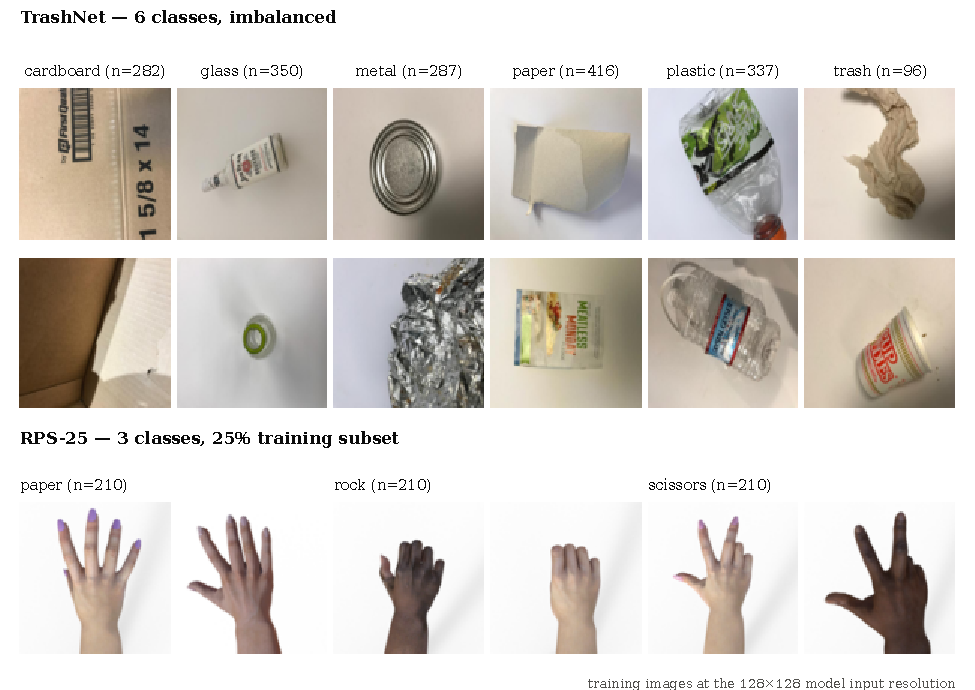
\includegraphics[width=\textwidth]{dataset_samples}
  \caption{Training images from the two datasets at the $128{\times}128$ input resolution, two per class, and the number of training images per class.}
  \label{fig:samples}
\end{figure*}

\begin{table*}[t]
  \centering
  \caption{Datasets and splits.}
  \label{tab:data}
  \adjustbox{max width=\textwidth}{\begin{tabular}{@{}lrrrrrll@{}}
\toprule
Dataset & Classes & Train & Val & Test & Smallest / largest train class & Train sampler & Primary metric \\
\midrule
TrashNet & 6 & 1{,}768 & 379 & 380 & trash 96 / paper 416 & class-balanced (weighted) & macro-F1 \\
RPS-25 & 3 & 630 & 33 & 372 & 210 / 210 (balanced) & shuffle & top-1 accuracy \\
\bottomrule
\end{tabular}
}
\end{table*}

\textbf{TrashNet}~\citep{yang2016trashnet} has \(2{,}527\) photographs in six classes (cardboard, glass, metal, paper, plastic, trash) and no official split.
We split it once, stratified $70/15/15$ with seed $0$, cache the split, and never re-split.
The classes are imbalanced (Table~\ref{tab:data}). Macro-F1 is therefore the primary metric, with accuracy as secondary, and training batches are drawn with a class-balanced sampler instead of class-weighted cross-entropy.
\textbf{RPS-25} is a $25\%$ subset of the training images of the Rock--Paper--Scissors dataset~\citep{moroney2019rps}. We chose it to be deliberately low-data so that distillation has room to help.
It keeps the official validation (33 images) and test (372 images) splits, and top-1 accuracy is its primary metric.
The two datasets differ in nature as well as size. RPS-25 is a three-class gesture task with clean backgrounds, and TrashNet is a six-class material task with imbalance. We treat RPS-25 as a low-data confirmation, not as a second application.
All images are resized to $128{\times}128$ and normalized with ImageNet statistics.
Training images use random resized crops, RandAugment~\citep{cubuk2020randaugment} and horizontal flips, with the strengths in Table~\ref{tab:hparams-students}. These are identical for every method.

\subsection{Teacher and students}
\label{sec:setup-models}

The teacher is an ImageNet-pretrained ResNet-50~\citep{he2016deep}, fine-tuned once per dataset and then frozen in evaluation mode with gradients disabled. Fine-tuning uses AdamW~\citep{loshchilov2019decoupled} with learning rate $10^{-4}$, weight decay $10^{-4}$, a cosine schedule, batch $128$, at most $20$ epochs and patience $5$, and selects by validation macro-F1.
Its test macro-F1 is \TeacherTn{} on TrashNet and \TeacherRps{} on RPS-25.
The students are trained from random initialization. They are MobileNetV2 with width multiplier $0.35$ (0.40\,M parameters), MobileNetV3-Small (0.93\,M) and a LeNet-5~\citep{lecun1998gradient} variant with global average pooling before the classifier (0.03\,M).
MobileNetV2-0.35 and MobileNetV3-Small are the edge-relevant students and the only ones exported. LeNet-5 serves as a capacity floor.

\subsection{Training protocol}
\label{sec:setup-training}

\begin{table*}[t]
  \centering
  \caption{Student recipes. BN: batch-normalization statistics are either the usual running estimates or the per-batch statistics used during training with a recalibration pass on clean training images before every evaluation (needed when an epoch has too few batches, or for MobileNetV3-Small's Hardswish and squeeze-excite blocks, to keep running statistics stable). RRC: minimum scale of the random resized crop. $^{*}$One of the three seeds used a different budget\extra{ (Appendix~\ref{app:recipe})}.}
  \label{tab:hparams-students}
  \adjustbox{max width=\textwidth}{\begin{tabular}{@{}llrrrcccc@{}}
\toprule
Dataset & Student & Epochs & Patience & LR & BN stats & RRC min scale & RandAugment (ops, mag.) \\
\midrule
TrashNet & MobileNetV2-0.35 & 60 & 10 & $0.001$ & running & 0.85 & 1, 5 \\
TrashNet & MobileNetV3-S & 40 & 8 & $0.001$ & per-batch + recal. & 0.85 & 1, 5 \\
TrashNet & LeNet-5 & 60 & 12 & $0.001$ & running & 0.85 & 1, 5 \\
RPS-25 & MobileNetV2-0.35 & 60 & 10 & $0.001$ & per-batch + recal. & 0.7 & 2, 9 \\
RPS-25 & MobileNetV3-S & 40 & 8 & $0.001$ & per-batch + recal. & 0.7 & 2, 9 \\
RPS-25 & LeNet-5 & 40/60$^{*}$ & 8/12 & $0.001$ & per-batch + recal. & 0.7 & 2, 9 \\
\bottomrule
\end{tabular}
}
\end{table*}

All methods on a pair share the data, the optimizer (AdamW, weight decay $10^{-4}$, cosine learning-rate schedule), the batch size ($128$), the epoch budget and the early-stopping patience (Table~\ref{tab:hparams-students}). The best validation checkpoint is restored.
Two cells depart from this\extra{ and are disclosed in Appendix~\ref{app:recipe}}. One \Scratch seed on RPS-25/LeNet-5 used a different budget, and the \Kd cell for that pair mixes two temperatures.
Checkpoints are selected by validation macro-F1 on TrashNet. On RPS-25 they are selected by validation loss, because the $33$-image validation split makes validation F1 too erratic to select on.
That validation loss is each method's own training objective evaluated on the validation batch. For the kernel methods it includes the kernel term at $\gamma_{\max}$, computed on a single $33$-image Gram matrix.
Each cell is trained with seeds $0$, $1$ and $2$, which set the student initialization, the data order and the random teacher projection.
Table~\ref{tab:hparams-methods} lists the loss settings that were used.

\begin{table*}[t]
  \centering
  \caption{Loss settings recorded in the runs. Kernel methods share $\tau=0.5$, whereas the \Kd temperature was screened on some pairs and reused on others (see text). $^{\P}$The seeds of this cell used different settings\extra{ (Appendix~\ref{app:recipe})}.}
  \label{tab:hparams-methods}
  \adjustbox{max width=\textwidth}{\begin{tabular}{@{}lll@{}}
\toprule
Method & Loss setting & Pairs \\
\midrule
\texttt{scratch} & CE$\times$1 & all pairs \\
\texttt{kd} & $\alpha{=}0.5$, $\beta{=}0.5$, $\tau{=}3$ & TrashNet (all students) \\
 & $\alpha{=}0.5$, $\beta{=}0.5$, $\tau{=}1$ & RPS-25: MobileNetV2-0.35, MobileNetV3-S \\
 & $\alpha{=}0.5$, $\beta{=}0.5$, $\tau{=}0.5$ & RPS-25: LeNet-5 (seed 0)$^{\P}$ \\
 & $\alpha{=}0.5$, $\beta{=}0.5$, $\tau{=}1$ & RPS-25: LeNet-5 (seeds 1, 2)$^{\P}$ \\
\texttt{rkd} & CE$\times$1, dist.$\times$5, angle$\times$10 & TrashNet: MobileNetV2-0.35, MobileNetV3-S; RPS-25: MobileNetV2-0.35, MobileNetV3-S \\
 & CE$\times$1, dist.$\times$1, angle$\times$2 & TrashNet: LeNet-5 \\
\texttt{rbf\_control} & $\alpha{=}0.5$, $\beta{=}0.5$, $\tau{=}0.5$, $\gamma{=}1$ (10-epoch ramp) & all pairs \\
\texttt{pqk} & $\alpha{=}0.5$, $\beta{=}0.5$, $\tau{=}0.5$, $\gamma{=}1$ (10-epoch ramp) & all pairs \\
\texttt{pqk\_adaptive} & $\alpha{=}0.5$, $\beta{=}0.5$, $\tau{=}0.5$, $\gamma{=}1$ (10-epoch ramp) & all pairs \\
\texttt{noent\_control} & $\alpha{=}0.5$, $\beta{=}0.5$, $\tau{=}0.5$, $\gamma{=}1$ (10-epoch ramp) & TrashNet: MobileNetV2-0.35, MobileNetV3-S; RPS-25: MobileNetV2-0.35, MobileNetV3-S \\
\bottomrule
\end{tabular}
}
\end{table*}

\subsection{Selection, reporting and the status of the results}
\label{sec:setup-protocol}

Every number is the mean $\pm$ sample standard deviation ($n{-}1$) over three seeds.
Comparisons are paired by seed. We report the mean paired difference, its standard deviation and the number of seeds on which the first method is ahead.
Two-sided paired $t$-tests are given as descriptive summaries and are not corrected for multiple comparisons.
For the follow-up arms (\texttt{pqk\_adaptive}, \texttt{noent\_control}, \texttt{pqk\_fit}, \texttt{rbf\_fit}) we checked that a shared seed means identical student initialization and data order, because the first-batch cross-entropy and KL gradients are identical across the arms. The stored gradient logs confirm this for \texttt{noent\_control}, \texttt{pqk\_fit} and \texttt{rbf\_fit} in every cell. For \texttt{pqk\_adaptive} the check was made when the arms were set up, and its logs were stored for two runs only.
For the earlier grid, pairing means a shared seed value only.

These results are exploratory, for three reasons.
First, several design choices were screened on seed~0, and some were judged by test-split scores. These are the student recipes (sampler, augmentation strength and epoch budget, tuned on MobileNetV2 for TrashNet), the KD temperature, and the RKD weights.
Second, the temperature of the kernel methods ($\tau=0.5$) was inherited from a KD screen on LeNet-5 with RPS-25 and was not re-tuned per pair. The \Kd temperature was screened on TrashNet/MobileNetV2-0.35 ($\tau=3$) and RPS-25/MobileNetV2-0.35 ($\tau=1$) and reused for the other students of the dataset (RPS-25/LeNet-5 is a special case\extra{, Appendix~\ref{app:recipe}}). Comparisons between a kernel method and \Kd are therefore not matched on that parameter, and may disadvantage the kernel methods.
Third, the choice of $\lambda$ for \Pqk was made after results were seen. The pre-specified $\lambda=1$ gave the \Pqk results of the first full grid. The adaptive $\lambda$ was adopted afterwards, per pair, by the higher three-seed \emph{validation} macro-F1 of the two variants\extra{ (Appendix~\ref{app:screens})}.
For the choice of $\lambda$ and for the follow-up analyses, validation scores decide and test scores are descriptive. The headline comparisons show both $\lambda$ variants.
A confirmatory claim would need a frozen protocol, selection on validation alone and fresh data, which we do not have.

\subsection{INT8 export}
\label{sec:setup-int8}

Each trained MobileNet student is exported in three steps. The projection and kernel modules are stripped, the PyTorch graph is converted to ONNX (opset 17, static batch size 1), and ONNX is converted to a fully integer TFLite model with per-channel weight quantization. Calibration uses $256$ unaugmented training images, and input and output are quantized to INT8.
Four checks run on every model: a purity check that the graph contains no projection, quantum or custom operations; a check that every convolution is quantized per channel and the whole graph is integer; ONNX--PyTorch parity on the logits; and reload of the fp32 weights reproducing the recorded test score.
The INT8 test score is measured with the LiteRT interpreter on an x86 PC, whose default and builtin kernels give identical outputs (``PC'' below).
The exported set contains $\NIntModels{}$ models: two students, two datasets, five methods and three seeds, plus the second $\lambda$ variant of \Pqk on the two pairs where both were exported.
For \Pqk the exported variant is the one the validation rule had chosen at export time. For TrashNet with MobileNetV2 that was $\lambda=1$, whereas the final rule prefers adaptive $\lambda$, which has no INT8 export (marked $\ddagger$ in the tables).

\subsection{On-device benchmark}
\label{sec:setup-device}

The INT8 models run on a Raspberry Pi~4 Model~B (Cortex-A72, four cores, 4\,GB, Ubuntu 20.04, \texttt{ondemand} governor, 600--1800\,MHz) with LiteRT (\texttt{ai-edge-litert} 2.1.0, Python 3.13).
Each model runs in a fresh process with $50$ warm-up and $500$ timed invocations at batch size~1, and every run starts below $55\,^\circ$C.
We log invocation latency percentiles, the full quantize--invoke--dequantize pipeline, load and cold-start time, CPU use, resident memory, and SoC temperature and clock every $100$\,ms. We also read the firmware's throttling flags before and after each timed window.
The suite covers all models with the default XNNPACK delegate and with the builtin kernels only, a thread sweep from one to four threads, and fp32 references.
Each model is also scored on the full test split on the device and compared with the PC's logits.
A live USB-camera pipeline ($640{\times}480$, MJPEG) measures the end-to-end cost including image preparation.
Energy was not measured because no power meter was attached, and the Jetson Orin Nano and ESP32-S3 targets were not benchmarked.

\subsection{Compute}
\label{sec:setup-compute}

All training ran on a single GPU, with several runs often sharing it. Per-epoch wall-clock times are therefore not comparable across methods, and we report compute-hours instead (Section~\ref{sec:results-cost}).
The $152$ student runs in the results include, besides the grid, the follow-up arms, the screens\extra{ of Appendix~\ref{app:screens}} and seven runs of two wider MobileNetV2 variants (width multipliers $0.5$ and $0.6$). Those seven were stopped as incomplete capacity probes and are not reported.
